\chapter{Entendimento do negócio}

  Com o aumento do número de viaturas (caminhões, ônibus, ambulâncias, carros, motos, barcos e helicópteros) do Corpo de 
  Bombeiros Militar do Distrito Federal (CBMDF), houve a necessidade de gerenciar com maior rigor e precisão.

  \begin{figure}[!htbp]
    \centering
    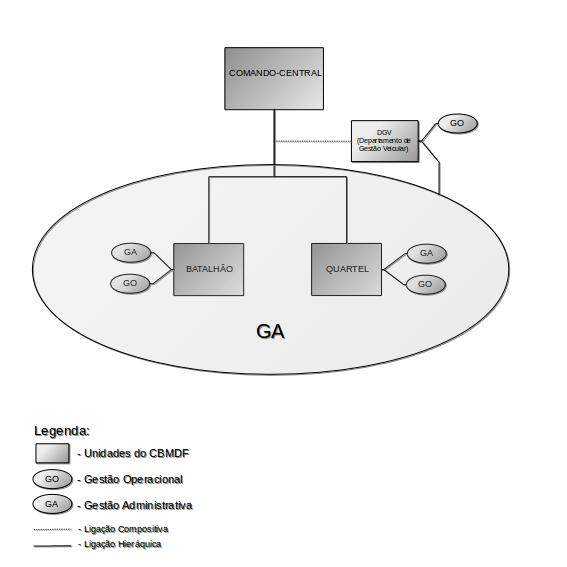
\includegraphics[scale=0.7, angle=0]{editaveis/figuras/entendimento_negocio}
    \caption{Organograma do CBMDF para o contexto de negócio.}
  \end{figure}
  
  A Figura 1 acima representa, organizacionalmente, as unidades do Corpo de Bombeiros Militar do Distrito Federal (CBMDF)
  envolvidas no contexto de negócio proposto para este projeto. As unidades estão dispostas hierarquicamente. 
  O Comando-Central é a unidade de maior escalão do CBMDF e, atualmente, possui grande dificuldade em obter uma ampla 
  visão das informações acerca de suas viaturas.
  
  \pagebreak

  O Departamento de Gestão Veicular (DGV) é a partição dentro do Comando-Central responsável pelo gerenciamento de todas 
  as viaturas da Corporação, incumbida da Gestão Administrativa de todo o CBMDF, no que diz respeito ao gerenciamento das 
  viaturas. Já as demais unidades (Batalhões e Quarteis) possuem a responsabilidade de gerenciar suas viaturas, de forma 
  independente, realizando as Gestões Administrativa e Operacional das viaturas inerentes à sua unidade.
  
  Cada unidade realiza as atividades das gestões administrativa e operacional independentemente e de forma despadronizada, 
  além de que todos os registros são feitos em planilhas eletrônicas, onde cada unidade possui suas próprias planilhas, 
  caracterizando uma descentralização das informações. Essa descentralização, falta das informações em tempo real, engessa 
  a comunicação entre as unidades e o DGV, este que tem que solicitar as informações para as unidades, juntá-las e interpretar 
  os dados para realizar a gestão administrativa das viaturas de toda a corporação.
  
  A gestão administrativa compreende as atividades de controle do custo do combustível, alocação das viaturas nas unidades
  (pelo DGV), acompanhamento da situação das viaturas e a gestão dos motoristas das unidades.
  
  A gestão operacional compreende as atividades no âmbito das operações realizadas pelas unidades, como o gerenciamento das 
  missões de uma unidade, vinculação de viaturas às missões, controle do consumo de combustível e verificação de 
  disponibilidade de viaturas.